\documentclass[paper=a4,fontsize=12pt,ngerman]{scrartcl}

\usepackage[utf8]{inputenc} 
\usepackage[T1]{fontenc}
\usepackage{graphicx}
\usepackage[ngerman]{babel}
\usepackage{amsmath}
\usepackage[a4paper,left=25mm,right=25mm,top=25mm,bottom=30mm]{geometry}
\usepackage{parskip}
\usepackage{url}
\usepackage{multirow}
\usepackage{tabularx}
\usepackage{paralist}
\usepackage{xcolor}
\usepackage{amssymb}
\usepackage{enumitem}

\usepackage[
colorlinks=true,
urlcolor=blue,
linkcolor=green
]{hyperref}
\definecolor{rosa}{HTML}{DF0174}

\newlist{titemize}{itemize}{1}% neue Listenumgebung für Tabellen
\setlist[titemize]{leftmargin=*,nosep,label=-}
% 


\begin{document}
	\pagenumbering{roman}
	\pagestyle{plain}
	
	% Einbinden der Titelseite
	
	\begin{titlepage}
	
	\linespread{1.5}
	
	
\includegraphics[width=\linewidth]{graphics/htw_logo}
	
	\begin{center}
		\large
		\hfill
		\vfill
		\Large{\bfseries{\textcolor{rosa}{Houdini Introduction\\ - \\ Prozedurale Modellierung}}}
		\\
		\large
		von \\
		Jana Koch, Laura Wagner, \\ 
		Nedim Thull, Ali Said, Samantha Maaß
		
	\end{center}
	
	\vfill
	
	
	\vfill
	
	%% {\bfseries{\textcolor{rosa}{}}}\\
	
	
	
	\vfill
\end{titlepage}

	\pagenumbering{arabic}
	\section*{\textcolor{rosa}{Getting started:}}
	\begin{itemize}
		\item Download der Free Test Version von Houdini 18.5.532 from https://sidefx.com/download/.
		\item Registrierung mit Username und E-Mail notwendig.
		\item Anmeldung auf der Webseite bevor Download möglich ist.
		\item Bei der Installation ist es ratsam, neben den bereits markierten Komponenten, direkt die 'SideFX Labs' zu installieren. Dies ist kein muss, spart allerdings Zeit falls man sie später doch benötigt. SideFX Labs ist ein Toolset zur Unterstützung von Aufgaben bei der Erstellung digitaler Inhalte. 
		\item Beim erstmaligen starten von Houdini muss eine Lizenz installiert werden, in unserem Fall die 'free Houdini Apprentice license'.
	\end{itemize}

	\section*{\textcolor{rosa}{Was ist Houdini?}}
		Houdini ist eine 3D-Grafiksoftware, deren Hauptaugenmerk auf der prozeduralen Modellierung liegt. Prozedurale Modellierung beschreibt mit Regeln, wie ein 3D-Objekt erzeugt werden soll. Sie können durch Attribute gesteuert werden und beschreiben Transformationen programmatisch. Dies wird in Houdini mit 'Nodes' realisiert. Sie beschreiben Aktionen die auf die Objekte angewendet werden und können miteinander zu einem 'Network' verknüpft werden. Dadurch lassen sich schnell sehr ähnliche aber einzigartige Objekte schaffen und immer wieder anpassen.  
		
	\section*{\textcolor{rosa}{Interface:}}
	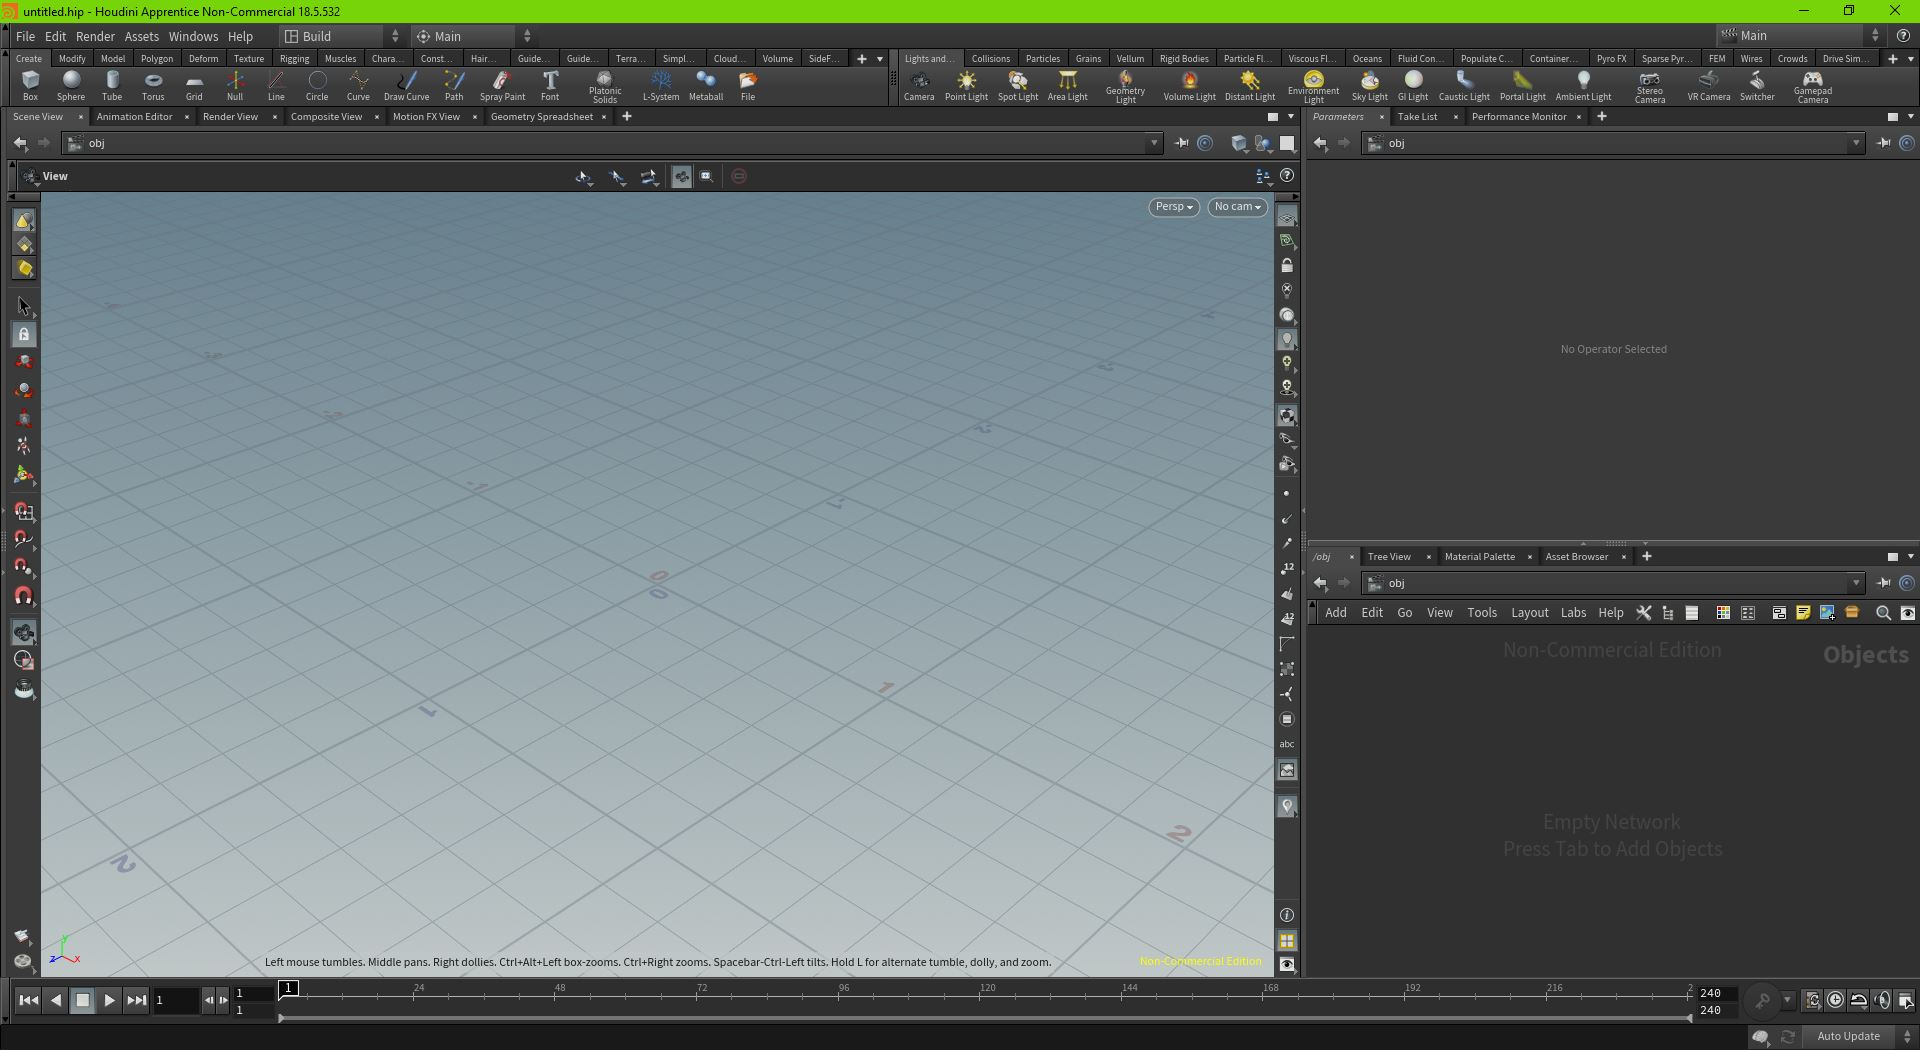
\includegraphics[width=\textwidth]{graphics/Interface.jpg}
	Das Standard-Interface ist in drei Teilbereiche aufgeteilt: 
	\begin{itemize}
		\item Die Scene View, eine 3D Ansicht der aktuellen Szene. (links)
		\item Der Parameter Editor, zum anpassen der Parameter der aktuell ausgewählten Node. (rechts oben)
		\item Der Network Editor, er zeigt alle Nodes des aktuellen Networks, man kann neue anlegen, sie miteinander verbinden und auswählen um die Parameter im Parameter Editor anzupassen. (rechts unten)
	\end{itemize}
	Die Panels können beliebig angepasst, und die Einstellungen gespeichert werden. Die Ansicht in der Scene View kann mit der Maus gesteuert werden: Linke Maustaste zum drehen, mittlere Maustaste zum verschieben und die rechte Maustaste oder das Mausrad zum zoomen. Es macht Sinn sich als erstes mit dem Interface vertraut zu machen, dazu haben wir uns hauptsächlich YouTube-Videos angeschaut. Besonders die 'Houdini isn't scary' - Tutorial Reihe von Nine Between (\url{https://youtu.be/Tsv8UGqDibc}) und die 'Getting started with Houdini' - Reihe von Arise.Works (\url{http://y2u.be/axD1ejlaEBA}) sind sehr zu empfehlen. Allerdings ist die Dokumentation von Houdini und die Tutorials von SideFX selbst sehr gut.
	
	\section*{\textcolor{rosa}{Tipps we wish we knew before:}}
	\begin{itemize}
		\item Mit 'Shift + Space + H' wird die Scene View wieder zurückgesetzt.
		\item Der Desktop kann komplett auf Standard zurück gesetzt werden, indem er neu geladen wird.
		\item Nodes können gruppiert, eingefärbt und in Subnetze unterteilt werden.
		\item 'Alle Wege führen nach Rom', aber es gibt immer einen Weg etwas schneller zu machen.
		\item Speichern. Oft.
		\item ESC spammen falls Attribute zu hoch - oder zu niedrig - gesetzt wurden kann einen Progammabsturz verhindern.
		\item Man kann im Parameter Editor die Node nach 'geänderten Parametern' durchsuchen: Lupe > Search All -> 'Parameters with Non-Default Values'
		\item Man kann die Panels auf mehrere Bildschirme verteilen: Pfeil in der rechten oberen Ecke des Panels > Tear off Pane Tab.
	\end{itemize}
		
\end{document}